\chapter{Enhancing Information Discovery and Curation Experience}
\label{chapter:improving}

Information discovery and curation enablers presented in the previous chapter are design elements that afford various operations. For example, the search feature affords typing in a query and searching. These operations can be further aided by another set of design elements. These design elements compose the second part of the conceptual framework for information discovery and curation titled \textit{``Enhancing Information Discovery and Curation Experience''} (see Figure~\ref{fig:framework_part2}). The primary goal of this part of the framework is to highlight opportunities for improvement over various information discovery and curation enablers.

Strategies for improvement include providing additional cognitive support for a given operation, personalizing user experience, and automating an operation. Not all of the strategies are feasible for every single operation. Some operations can be supported in multiple ways. The following sections outline some of the possibilities for for advancing information discovery and curation features. 
 
\begin{figure}[ht!]
	\noindent
	\centering
	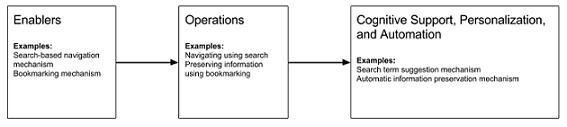
\includegraphics[width=\linewidth]{framework_part2.png}
	\caption{Framework Overview (Part II): Enhancing Information Discovery and Curation Experience}
	\label{fig:framework_part2} 
\end{figure}

{\section{Enhancing Navigation}
There are two common methods of enhancing information discovery when search-based navigation is used (see Table~\ref{table:navigation_support}). The first method entails returning personalized results when the user enters a search query. Personalization can be accomplished using a variety of techniques, including predefined user preferences, social interactions, context, browsing history, etc. The second method is to suggest search terms to make it easier for the user to formulate the information need. For example, Yelp suggests search terms as the user enters their query.

To further support referential navigation, applications can personalize reference suggestions, such as categories, tags, and topics of interest. They can also suggest relevant resources based on the one that the user already picked. As an example, Pinterest showcases similar `pins' once the user clicks on any of them.

For opportunistic navigation, Web tools sometimes allow users to personalize types or categories of information that they the users would like to discover. StambleUpon allows to not only choose topics of interests, but it can also help discover new topics that might be promising for the user.

Featured content can also be personalized to improve information discovery with system-regulated navigation. For example, Yelp showcases restaurants from a predefined area, such as the city where the user is from.

Finally, to make better use of subscribed content and reduce human efforts in information search, an application can support various notification mechanisms. These mechanisms can advise the user about updates on the website content, various artifacts, and activities of other users.  

\begin{table}[ht!]
\caption{Cognitive Support, Automation, and Personalization for Navigation}
\label{table:navigation_support}
\begin{tabular}{{|p{0.35\linewidth}|p{0.60\linewidth}|}}
\hline
Support, automation, and personalization elements & Questions to be posed during the design or evaluation of discovery and curation tools \\
\hline
\textbf{Descriptional}       & \\
Personalized results         & Does the search mechanism return personalized results? \\
Guided search                & Does the system suggest search terms to the user? \\
\textbf{Referential}         & \\
Suggesting categories & Does the system suggest categories of interest? \\
Suggesting topics of interest & Does the system suggest topics of interest? \\
Suggesting tags              & Does the system suggest similar tags? \\
Suggesting similar resources & Does the system suggest similar resources? \\
\textbf{Opportunistic} & \\
Personalized opportunistic navigation     & Is it possible to personalize opportunistic navigation? \\
\textbf{System-regulated} & \\
Personalized featured content         & Is featured content personalized to the user? \\                                                       
User activity update notification & Is it possible to receive notifications about other users' activities? \\
Application activity update notification & Is it possible to receive notifications about website content updates?\\
Artifact update notification & Is it possible to receive notifications about artifact-related updates? \\                                                       
\hline

\end{tabular}
\end{table}


} % end subsection
{\section{Enhancing Exploration}
Personalization in spatial information representation usually has limited support in Web applications. Presumably, it is because consistency is more welcomed within information discovery applications than spatial personalization. However, it is still a possibility to personalize how multiple resources or information within a single resource are arranged (see Table~\ref{table:exploration_support}). For instance, users can rearrange songs in a YouTube playlist although this operation has mostly functional nature.

Visual and textual personalizations are more common, especially when the content within the application is curated by its users.  For example, a Web application for tracking personal goals, BucketList, allows its users to personalize how their goals look, so that it is easier to rediscover information. Similarly, `pinboards' on Pinterest can have personalized cover images.

\begin{table}[ht!]
\caption{Visual and Spatial Exploration Cognitive Support and Personalization}
\label{table:exploration_support}
\begin{tabular}{{|p{0.33\linewidth}|p{0.62\linewidth}|}}
\hline
Cognitive support and personalization design elements & Questions to be posed during the design or evaluation of discovery and curation tools  \\
\hline
\textbf{Visual and textual cues of multiple resources} & \\
Personalized visual preview  & Is it possible to personalize visual previews of resources? \\
Personalized textual preview & Is it possible to personalize textual previews of resources? \\
\textbf{Visual and textual cues of a single resource} & \\
Personalized visual cues                 & Is it possible to personalize the visual cues within a resource? \\
Personalized textual cues                & Is it possible to personalize the textual cues within a resource? \\
\textbf{Spatial proximal cues of multiple resources} & \\
Personalized arrangement of multiple resources & Is it possible to personalize the arrangement of resources? \\                                                    
\textbf{Spatial proximal cues of a single resource} & \\
Personalized arrangement of information within a resource          & Is it possible to personalize the arrangement of information within a resource? \\                                                       
\hline
\end{tabular}
\end{table}
} % end subsection

{\section{Enhancing Curation}

\begin{table}[ht!]
\caption{Cognitive Support, Personalization, and Automation for Curation}
\label{table:curation_support}
\begin{tabular}{{|p{0.30\linewidth}|p{0.65\linewidth}|}}
\hline
Cognitive support, personalization, and automation elements & Questions to be posed during the design or evaluation of information discovery and curation tools \\
\hline
\textbf{Management}		& \\
Suggesting collections  & Does the system suggest relevant collections? \\
Suggesting tags         & Does the system suggest relevant tags? \\
Automated classification into collections  	& Does the system automatically sort resources into collections? \\
Automated tagging       & Does the system automatically tag resources? \\
\textbf{Preservation}   & \\
History       			& Does the system automatically preserve information found by the user? \\
Suggested preservation  & Does the system suggest preservation channels to the user? \\
\textbf{Augmentation} 	& \\
Automated augmentation  & Does the system automatically annotate resources? \\
Suggested augmentation  & Does the system suggest annotation options to the user? \\    
\textbf{Sharing}        & \\
Automated sharing		& Does the system support automatic sharing? \\
Suggested sharing		& Does the system suggest sharing channels to the user? \\
\textbf{Subscription}   & \\
Suggesting users for subscription & Does the system suggest which users to subscribe to? \\
Suggesting artifacts for subscription   & Does the system suggest which artifacts to subscribe to? \\ 
Automated subscription  & Can the system subscribe the user automatically to the website activity? \\
&\\
\hline  
\end{tabular}
\end{table}

Management of information can be improved if the system helps the user make decisions about information categorization or tagging (see Table~\ref{table:curation_support}). Alternatively, information can be categorized or tagged automatically. For example, when the user bookmarks a restaurant on Yelp, it is automatically categorized. The user can filter bookmarks by category whenever they go into the embedded bookmark manager. \\

Preservation operations can also be automated. An example of the most common automatic preservation mechanism is history. Many applications, such as YouTube and Google Maps, preserve users' browsing history so that they can review it later. Additionally, preservation mechanisms can be suggested to the user.

YouTube allows users to automatically share information about their activities, such as comments,  added videos, liked or disliked videos, and created playlists. In general, socially curated spaces offer sharing channels to support convenient information communication.
 
Augmentation is another aspect of information curation that can be either automated or suggested to the user. For example, Yelp asks to rate places which the application identifies as visited by the user. 

Notification mechanisms enable user awareness about new content on the subscribed channel~\cite{millen2005social}. Web applications, that facilitate rapidly updating content, support various notification mechanisms, such as messages within the application, informative emails, and smartphone notifications. Many types of notifications include suggestions of users or artifacts to follow. Some Web tools subscribe users to their notifications automatically, usually along with registration.\\
} % end subsection

Providing cognitive support, personalization, and automation dramatically improves user experience when they interact with information discovery and curation systems. Using the information discovery factors in my framework, I described and evaluated currently existing tools. Similarly, the framework can be used for identifying gaps in information discovery support and developing new technologies (see Chapters~\ref{chapter:application} and~\ref{chapter:evaluation}).  